\chapter{LLM-Driven Data Augmentation for Visual Question Answering}
\epigraph{\itshape  La volonté trouve, la liberté choisit. Trouver et choisir, c'est penser}{-- Victor Hugo}

\startcontents[chapters]
\printmyminitoc{
	%\lipsum[1]
}


%\def\BibTeX{{\rm B\kern-.05em{\sc i\kern-.025em b}\kern-.08em
    %T\kern-.1667em\lower.7ex\hbox{E}\kern-.125emX}}

%\title{LLM Augmentation for Robust RSVQA}
%\title{LLM-Driven Data Augmentation for Visual Question Answering}



%\author{\IEEEauthorblockN{Hichem Boussaid, Nayoung Kwon, Camille Kurtz, Laurent Wendling, Sylvain Lobry}
%\IEEEauthorblockA{\textit{LIPADE, Université Paris Cité, 75006 Paris, France}}
%firstname.lastname@u-paris.fr}

%\maketitle

%\ck{le titre est vraiment trop proche du papier concurrent : Multilingual Augmentation for Robust Visual Question Answering in Remote Sensing Images}

%\ck{Quelques articles récents pour compléter ton SOA : https://www.sciencedirect.com/science/article/pii/S1077314223002424

%https://www.ecva.net/papers/eccv_2022/papers_ECCV/papers/136960094.pdf

%https://aclanthology.org/2024.eacl-srw.20.pdf

% et un survey
%https://export.arxiv.org/pdf/2401.15422
%https://github.com/MLGroup-JLU/LLM-data-aug-survey
%}
\section{Introduction}
\label{sec:chap3_intro}
% ============================================================
 
Despite growing interest in RSVQA, a fundamental limitation
persists across existing approaches: poor generalization to unseen
question formulations. Most RSVQA datasets are automatically
generated from geospatial vectorial databases such as OpenStreetMap~\cite{openstreetmap}\cite{lobry2020rsvqa},
which results in a limited set of question
templates. Models trained on such data learn to exploit
surface-level linguistic patterns rather than developing a robust
understanding of the underlying visual content. As a
consequence, even semantically equivalent questions,
differing only in wording or syntactic structure, can lead to
dramatically different model predictions. This phenomenon,
known as linguistic bias, has been identified as a critical
obstacle to the deployment of RSVQA systems in real-world
scenarios where users formulate queries freely and
unpredictably~\cite{chappuis2023curse}.
 
It is worth noting that this work was conducted at a time when
RSVQA models predominantly relied on a dual-encoder
architecture, a visual encoder such as ResNet~\cite{he2015deepresiduallearningimage} or a Vision
Transformer~\cite{dosovitskiy2021imageworth16x16words})
paired with a text encoder such as BERT~\cite{sanh2020distilbertdistilledversionbert},
 followed by a fusion module for answer prediction. In this
paradigm, the model has no generative capacity and no world
knowledge beyond what is encoded in its training data, making
it particularly sensitive to the linguistic distribution of the
training questions. The recent shift toward large
vision-language models with generative capabilities has
partially alleviated this problem by leveraging pre-training on
massive and diverse corpora. However, at the time of this
work, such models were not yet established in the remote
sensing domain, and the challenge of linguistic generalization
in RSVQA remained largely unaddressed. The contribution
presented in this chapter should therefore be understood in
this context: a targeted, data-centric approach to improve
robustness within the then-dominant encoder-based RSVQA
framework.
 
Data augmentation is a natural strategy to address this
limitation. Two approaches have been widely studied in the
natural language processing literature: paraphrasing and back
translation. Paraphrasing involves rewriting a sentence while
preserving its meaning, but rule-based methods often fail to
capture the full range of linguistic variation and do not scale
to large datasets~\cite{bhagat2013paraphrase}. Back
translation, translating a question into an intermediate
language and then back into the original, offers a scalable
alternative~\cite{yuan2023multilingual}. However, it tends to
produce questions that remain structurally close to the
original, limiting the diversity of the augmented dataset.
Furthermore, translation quality varies depending on the
language pair and domain vocabulary, which can introduce
noise into the training data.
 
The emergence of Large Language Models (LLMs) offers a
fundamentally new perspective on this problem. Models such
as LLaMA-2~\cite{touvron2023llama2openfoundation}, trained on massive
corpora with instruction-following capabilities, can generate
diverse, coherent, and semantically faithful reformulations of
a given question with minimal supervision. Unlike back
translation, LLM-based paraphrasing is not constrained by the
structure of a pivot language and can produce syntactically
varied outputs while preserving the semantic content and
expected answer. This makes LLMs particularly well-suited
for the RSVQA augmentation problem, where the goal is to
expose the model to a wide variety of question formulations
without altering the ground truth.
 
In this chapter, we propose a data augmentation framework
based on LLMs to improve the robustness and generalization
of RSVQA models. Concretely, we use LLaMA-2-7B to
generate ten semantically equivalent reformulations of each
question in the RSVQA-HR dataset~\cite{lobry2020rsvqa},
guided by a prompt selected through systematic evaluation of
nine candidates across questions of varying linguistic
complexity. We compare this approach against back translation
and evaluate both in terms of in-distribution performance and
generalization to unseen question formulations.
 
The remainder of this chapter is organized as follows.
Section~\ref{sec:chap3_rw} reviews related work on data
augmentation for VQA and the use of LLMs for text
generation. Section~\ref{sec:chap3_method} presents the
proposed augmentation methodology.
Section~\ref{sec:chap3_experiments} details the experimental
setup and results. Section~\ref{sec:chap3_conclusion} concludes
the chapter and discusses limitations and perspectives.

\section{Related Work}
\label{sec:chap3_rw}

\subsection{Data Augmentation in Natural Language Processing}
\label{sec:chap3_rw_nlp}
 
Data augmentation in NLP aims to increase training data
diversity without new annotations, improving model
robustness and reducing overfitting. Early work focused
on simple rule-based token-level operations.
\cite{wei2019eda} proposed Easy Data Augmentation (EDA),
consisting of four lightweight operations: synonym
replacement, random insertion, random swap, and random
deletion, that improved performance on text
classification tasks, especially in low-resource settings.
Despite their simplicity, these operations suffer from a
fundamental limitation: modifications are local and may
introduce semantic inconsistencies for complex or
domain-specific sentences. In the RSVQA context, where
questions involve spatial relations and domain vocabulary
(\textit{e.g.}, \textit{``at the bottom of a rectangular
commercial building''}), such perturbations can 
corrupt the intended meaning entirely.
 
Back translation, originally proposed by
\cite{sennrich2016backtranslation} for neural machine
translation, offers a more principled alternative: a
source sentence is translated into a pivot language and
then back into the original, yielding a paraphrase that
preserves meaning while introducing new surface forms.
\cite{edunov2018backtranslation} later studied this
approach at scale, confirming its benefits across
generation tasks. However, back translation is
constrained by the quality of the underlying translation
system and tends to produce output that remains
structurally close to the original, as the pivot language
acts as a bottleneck on syntactic diversity. For questions
involving rare or domain-specific terms, translation
quality degrades further, potentially introducing noise
into training data.
 
\subsection{Data Augmentation for VQA and RSVQA}
\label{sec:chap3_rw_vqa}
 
Language bias is a well-documented problem in VQA: models
trained on datasets with skewed answer distributions
learn to exploit statistical shortcuts in questions rather
than performing genuine visual reasoning. Data augmentation
has emerged as a primary strategy to mitigate this.
\cite{gokhale2020seada} introduce Semantic Equivalent
Adversarial Data Augmentation (SEADA), generating
adversarial question paraphrases using syntactically
controlled paraphrase networks, showing improved VQA
robustness to linguistic variation.
\cite{sheng2021contrastclassify} propose a contrastive
training objective that explicitly encourages VQA
representations to be invariant to question rephrasing,
achieving gains on the VQA-Rephrasings benchmark which
evaluates answer consistency across human-written
paraphrases. \cite{chen2022rethinkingDA} propose KDDAug,
a knowledge distillation-based augmentation framework
that generates new image-question pairs and assigns
pseudo-answers via a teacher model, improving robustness
across question types without human-designed rules.
 
In the remote sensing domain specifically, the
generalization problem is more severe than in standard
VQA. \cite{chappuis2023curse} provide a systematic
analysis through visual-blind models and adversarial
testing, showing that RSVQA models rely heavily on
linguistic shortcuts and that biases stem from the
automatic and template-based question generation
strategies used in existing RS datasets.
\cite{yuan2023adversarial} address this from the model
side, introducing an adversarial training framework with
regularizers to reduce language bias in RSVQA.
The most directly related augmentation work is that of
\cite{yuan2023multilingual}, who apply back translation
to RSVQA questions via Chinese, German, and French as
pivot languages, combined with a contrastive learning
strategy to train more robust representations. While
effective, this approach is limited by the structural
proximity of back-translated questions to their originals
and by translation quality degradation on RS-specific
vocabulary. The work presented in this chapter directly
addresses these limitations by replacing back translation
with LLM-driven generation, which produces more
syntactically diverse reformulations while maintaining
semantic fidelity.
 
\subsection{Large Language Models for Paraphrasing and Question Generation}
\label{sec:chap3_rw_llm}
 
The use of LLMs for controlled paraphrasing and text
generation has grown rapidly with instruction-tuned
models. Unlike back translation, LLM-based paraphrasing
is not constrained by a pivot language and can be guided
through natural language prompts to enforce specific
constraints, making it
particularly suited to the RSVQA augmentation setting.
 
\cite{meng2022lmcppf} demonstrate that few-shot
paraphrasing with large language models such as GPT-3
outperforms both EDA and back translation for
augmentation in text classification, with stronger
semantic fidelity in generated examples.
\cite{dai2023llmaugsurvey} provide a comprehensive
survey of LLM-based augmentation strategies, identifying
paraphrasing, question generation, and counterfactual
rewriting as the most impactful approaches, and
highlighting the role of prompt design in controlling
output quality. \cite{whitehouse2023llmcrosslingual}
further show that LLM-powered augmentation transfers
effectively across languages and low-resource domains
where back translation typically fails. These results
collectively motivate our use of
LLaMA-2~\cite{touvron2023llama2openfoundation} as the generation
backbone: it offers strong instruction-following
capabilities at a manageable scale (7B parameters),
making it suitable for generating large volumes of
question reformulations without the computational and
financial cost of proprietary models such as GPT-4.
 

\section{Methodology}
\label{sec:chap3_method}
% ============================================================
 
This section describes the proposed framework for
augmenting RSVQA datasets using Large Language Models.
The goal is to generate semantically equivalent
reformulations of existing questions in order to expose
RSVQA models to a wider variety of phrasings during
training, thereby improving their robustness to unseen
question formulations.
 
\subsection{Problem Formulation}
\label{sec:chap3_formulation}
 
Let $\mathcal{Q} = \{q_1, q_2, \ldots, q_n\}$ be a set
of $n$ input questions from a given RSVQA dataset, where
each question $q_i$ is associated with a ground truth
answer $a_i$. The goal of our augmentation framework is
to generate a set of rephrased questions
$\mathcal{Q}' = \{Q'_1, Q'_2, \ldots, Q'_n\}$, where
each $Q'_i$ corresponds to a set of rephrased versions
of $q_i$:
 
\begin{equation}
    Q'_i = \{q'^1_i, q'^2_i, \ldots, q'^r_i\}
\end{equation}
 
such that for all $q' \in Q'_i$, the semantic meaning
of $q'$ is equivalent to $q_i$ and the ground truth
answer is preserved (\textit{i.e.}, $a'_i = a_i$),
while the syntactic structure differs. This formulation is different from standard
data augmentation in computer vision, where transformations
are applied directly to the input signal: here, the
constraint is purely semantic: a generated question
is valid if and only if a human annotator would give
the same answer as to the original.
 
\subsection{LLM Selection}
\label{sec:chap3_llm_selection}
 
We use LLaMA-2-7B~\cite{touvron2023llama2openfoundation} as the
generation model. Several considerations motivated
this choice.
 
\textbf{Instruction-tuned models.} Generating
semantically faithful paraphrases requires the model
to follow precise instructions (\textit{e.g.}, ``preserve
the meaning'', ``return only questions''). Base language
models, optimized for next-token prediction without
instruction fine-tuning, are poorly suited for this: they
tend to continue the question rather than rephrase it, or
produce outputs that mix questions and explanations. We
therefore restrict our selection to instruction-tuned
variants of open-source models.
 
\textbf{Model scale.} LLaMA-2 is available in three
sizes (7B, 13B, 70B parameters). While larger models
generally produce higher-quality text, the 7B variant
offers a practical trade-off between generation quality
and computational cost for our use case, which requires
generating reformulations for hundreds of thousands of
questions. The 7B model fits on a single GPU and produces
outputs at a speed that makes large-scale augmentation
feasible.
 
\textbf{Reproducibility and cost.} Proprietary models
such as GPT-3.5 or GPT-4 could also be used for this
task, and would likely produce high-quality paraphrases.
However, their use raises concerns about reproducibility
(outputs may change between API versions) and cost
(generating augmented versions of a dataset with nearly
one million question-answer pairs at API pricing is
prohibitive). LLaMA-2 is fully open-source, runs
locally.
 
\subsection{Prompt Engineering}
\label{sec:chap3_prompts}
 
The quality of LLM-generated paraphrases is highly
sensitive to the formulation of the input prompt. We
designed a set of $k = 9$ distinct prompts
$\mathcal{P} = \{p_1, p_2, \ldots, p_9\}$, each
instructing the model to generate exactly 10 rephrased
versions of a given question. The prompts were designed
to explore different axes of variation:
 
\begin{itemize}
    \item \textbf{Instruction verb}: some prompts use
    \textit{generate}, others use \textit{rephrase},
    \textit{find ways to ask}, or \textit{create},
    which influences the model's generation strategy.
 
    \item \textbf{Answer-awareness}: some prompts
    ($p_4$, $p_9$) explicitly provide the ground truth
    answer as context, asking the model to generate
    questions that share the same answer. Others only
    provide the question, leaving answer preservation
    implicit.
 
    \item \textbf{Output format constraints}: some
    prompts impose a strict numbered format
    (\textit{e.g.}, ``1.<question> 2.<question>...''
    in $p_6$, $p_7$, $p_9$) to facilitate parsing,
    while others leave the format open.
 
    \item \textbf{Semantic framing}: some prompts
    emphasize \textit{same meaning} ($p_1$, $p_6$,
    $p_8$), others emphasize \textit{same semantic
    but different syntax} ($p_5$, $p_7$), reflecting
    different intuitions about what constitutes
    a valid paraphrase.
\end{itemize}
 
The full set of prompts and their associated keywords
is summarized in Table~\ref{tab:prompts}.
 
\begin{table*}[!t]
  \centering
  \footnotesize
   \resizebox{\textwidth}{!}{ % Adjust the width as needed
    \begin{tabular}{|c|c|c|}
    \hline
     & \textbf{Prompts}  & \textbf{keywords}\\
    \hline
    p1 & Generate exactly 10 different questions based on: \{question\}. New questions should have the same  &Generate, meaning\\
    &meaning as the initial question&\\
    \hline
    
    p2 & Find exactly 10 different ways to ask:\{question\}. New questions should have the same answer &Find, ways\\
    &as the initial question but return only questions and not answers.&\\
    \hline
    
    p3 & I am doing a Visual Question Answering project. I already have a dataset with questions and&Visual Question\\
    &corresponding answers. I want you to generate exactly 10 questions based on a given question that &Answering,\\ 
    &already exists which is \{question\}. You should only return generated 10 questions and nothing else.&generate\\
    \hline
    
    p4 & Generate exactly 10 different questions based on: {question}. New questions should have the same &Generate,\\
    &meaning as the initial question. All the questions should have the same answer which is {answer}.&meaning,\\
    &Print generated questions only.&answer\\
    \hline

    p5 & I have the question {question}. Create exactly 10 more questions which have the same semantic but&Semantic, \\
    &different syntax. Do not return anything other than he generated questions.&syntax\\
    \hline

    p6 & Create 10 questions with the same meaning but different wording as the following&Create, meaning,\\
    &question:\{question\}. Use the following format : 1.\textless{}question created\textgreater{} 2.\textless{}question created\textgreater{}&wording, format\\
    &3.\textless{}question created\textgreater{} 4.\textless{}question created\textgreater{} 5.\textless{}question created\textgreater{} 6.\textless{}question created\textgreater{}&\\ 
    &7.\textless{}question created\textgreater{} 8.\textless{}question created\textgreater{} 9.\textbf{}question created\textgreater{} 10.\textless{}question created\textgreater{}&\\
    \hline

    p7 & Create 10 questions with the same semantic but different syntax as the following \{question\}.&Create, semantic,\\
    &Use the following format : 1.\textless{}question created\textgreater{} 2.\textless{}question created\textgreater{} 3.\textless{}question created\textgreater{}&syntax,\\
    & 4.\textless{}question created\textgreater{} 5.\textless{}question created\textgreater{} 6.\textless{}question created\textgreater{} 7.\textless{}question created\textgreater{}&format\\ 
    & 8.\textless{}question created\textgreater{} 9.\textbf{}question created\textgreater{} 10.\textless{}question created\textgreater{}&\\
    \hline

    p8 & Rephrase the question \{question\} to ask about the same thing in exactly 10 different ways.&Rephrase, thing,\\ 
    &New questions should have the same meaning.&ways, meaning\\
    \hline

    p9 & The initial question is \{question\}. Generate exactly 10 questions based on the initial question.&Generate,\\
    &Generated questions should have the same meaning but different wording as the initial question.&wording, answer,\\ 
    &Also, generated questions should have the same answer as \{answer\}. Use the following format :&format,meaning\\
    &1.\textless{}question created\textgreater{} 2.\textless{}question created\textgreater{}3.\textless{}question created\textgreater{} 4.\textless{}question created\textgreater{}&\\ 
    &5.\textless{}question created\textgreater{} 6.\textless{}question created\textgreater{} 7.\textless{}question created\textgreater{} 8.\textless{}question created\textgreater{}&\\ &9.\textbf{}question created\textgreater{} 10.\textless{}question created\textgreater{}&\\
    \hline

  \end{tabular}
  }
  \caption{Summary of prompts used for question generation, along with their associated keywords. Each prompt (p1–p9) describes a method for creating questions based on a given question (\{question\}) and, where applicable, an answer (\{answer\}). The keywords highlight key elements such as "Generate," "Semantic," and "Wording,".}
  \label{tab:prompts}
\end{table*}



\subsection{Difficulty Grouping and Prompt Evaluation}
\label{sec:chap3_difficulty}
 
To evaluate the quality of generated questions, we
first classified the input questions $\mathcal{Q}$
into three difficulty levels based on their structural
and linguistic complexity:
 
\begin{equation}
d(q_i) =
\begin{cases}
\text{easy,}   & \text{if } q_i \text{ involves a single element} \\
\text{medium,} & \text{if } q_i \text{ involves multiple elements} \\
\text{hard,}   & \text{if } q_i \text{ involves complex relations or attributes}
\end{cases}
\end{equation}
 
This taxonomy reflects the observation that question
complexity has a direct impact on the difficulty of
generating faithful paraphrases: single-element
questions (\textit{e.g.}, \textit{``Is there a road?''})
are easy to rephrase while preserving meaning, whereas
questions involving spatial relations between multiple
objects (\textit{e.g.}, \textit{``Is a park at the bottom
of a rectangular commercial building present?''}) pose
a significantly greater challenge for the model.
 
For each of the 9 prompts, we manually evaluated the
generated questions on a representative subset of
questions from each difficulty level. Each generated
question was classified as \textit{correct}
(semantically equivalent to the original, same answer),
\textit{borderline} (meaning slightly altered but
arguably equivalent), or \textit{incorrect} (meaning
changed or answer not preserved). The results of this
evaluation are presented in Table~\ref{tab:prompt_eval}.

\begin{table*}[!t]
  \centering
  \footnotesize
   \resizebox{\textwidth}{!}{ % Adjust the width as needed
    \begin{tabular}{|c|c|c|c|c|c|c|c|c|c|c|}
    \hline

    && \multicolumn{9}{c|}{number of correct/incorrect/borderline questions} \\ \cline{3-11}

     Complexity&Question& \textbf{p1}  & \textbf{p2}& \textbf{p3}& \textbf{p4}& \textbf{p5}& \textbf{p6}& \textbf{p7}& \textbf{p8}& \textbf{p9}\\
    \hline


    \multirow{2}{*}{Easy} & Is there a road? & 3/6/1 & 4/5/1 & -/10/- & 3/7/- & -/10/- & -/10/- & 5/2/3 & 2/4/4 & 5/4/1\\
    \cline{2-11}
    
    &Is a water area present in the image? & -/3/- & 10/-/- & 1/9/- & 6/5/1 & 9/1/- & 10/-/- & 10/-/- & 10/-/- & 10/-/-\\
    \hline

    \multirow{2}{*}{Medium}&Is there a medium park in the image? & 9/1/- & 9/-/1 & -/10/- & 5/3/2 & 1/6/3 & 8/2/- & 10/-/- & 10/-/- & -/10/- \\
    \cline{2-11}

    &Are there more roads than parks? & 2/7/1 & 2/8/- & -/10/- & -/10/- & 1/9/- & 5/4/1 & 4/6/- & 5/5/- & 2/8/-\\
    \hline

    \multirow{2}{*}{Hard}&What is the area covered by grass areas  & 1/9/- & 3/6/1 & -/10/- & 4/6/- & 6/1/3 & 6/2/2 & -/10/- & 6/1/3 & 4/6/-\\
    &at the bottom of a  road in the image? &  &  &  &  &  &  &  &  & \\ 
    \cline{2-11}
    &Is a park at the bottom of a  rectangular  & 1/9/- & 1/9/- & -/10/- & -/10/- & -/9/- & 4/6/- & 6/4/- & 5/5/- & -/10/-\\
    &commercial building present? &  &  &  &  &  &  &  &  & \\ 
    \hline
    \hline
    \multirow{4}{*}&Correct & 23 & 29 & 1 & 16 & 18 & 33 & 35 & 38 & 21\\
    \cline{2-11}
    &Incorrect & 35 & 28 & 59 & 41 & 36 & 24 & 22 & 15 & 38\\
    \cline{2-11}
    &Borderline & 2 & 3 & 0 & 3 & 6 & 3 & 3 & 7 & 1\\
    \cline{2-11}
    &Accuracy (\%) & 38.3 & 48.3 & 1.7 & 26.7 & 30 & 55 & 58.3 & 63.3 & 35\\
    \hline

  \end{tabular}
  }
  \caption{Performances of different prompts (p1–p9) (see Table \ref{tab:prompts}) in answering questions across Easy, Medium, and Hard complexities. The numbers represent correct/incorrect/borderline responses for each question.}
  \label{tab:perf prompts}
\end{table*}
 
 
The optimal prompt $p^*$ was selected as:
 
\begin{equation}
    p^* = \arg\max_{p_j \in \mathcal{P}} \text{Qual}(p_j)
\end{equation}
 
where $\text{Qual}(p_j)$ measures the proportion of
correct generated questions across all difficulty levels.
From this evaluation, prompt $p_8$ (\textit{``Rephrase
the question \{question\} to ask about the same thing
in exactly 10 different ways. New questions should have
the same meaning.''}) achieved the highest accuracy
(63.3\%), followed by $p_7$ (58.3\%) and $p_6$ (55.0\%).
Prompt $p_3$, which used Visual Question Answering
framing and imposed no format constraints, performed
worst (1.7\%), generating answers rather than questions
in most cases. These results highlight the critical
importance of prompt formulation: small changes in
wording can lead to dramatically different generation
behaviors.
 
\subsection{Final Augmentation Pipeline}
\label{sec:chap3_pipeline}
 
Given the optimal prompt $p^*$, the final augmented
dataset is generated as follows. For each unique
question $q_i$ in the dataset, we generate a set of
$r = 10$ rephrased questions:
 
\begin{equation}
    \mathcal{Q}' = \bigcup_{i=1}^{n} \{M(q_i, p^*)\}
\end{equation}
 
where $M$ denotes the LLaMA-2-7B model. Augmented
questions are then added to the dataset by replacing
each occurrence of $q_i$ in the training, validation,
and test sets with the union of $q_i$ and its
10 reformulations $Q'_i$. This results in a dataset
approximately 10 times larger than the original,
with the same image-answer associations and a
significantly richer distribution of question phrasings.
 
\begin{figure}[ht]
  \centering
  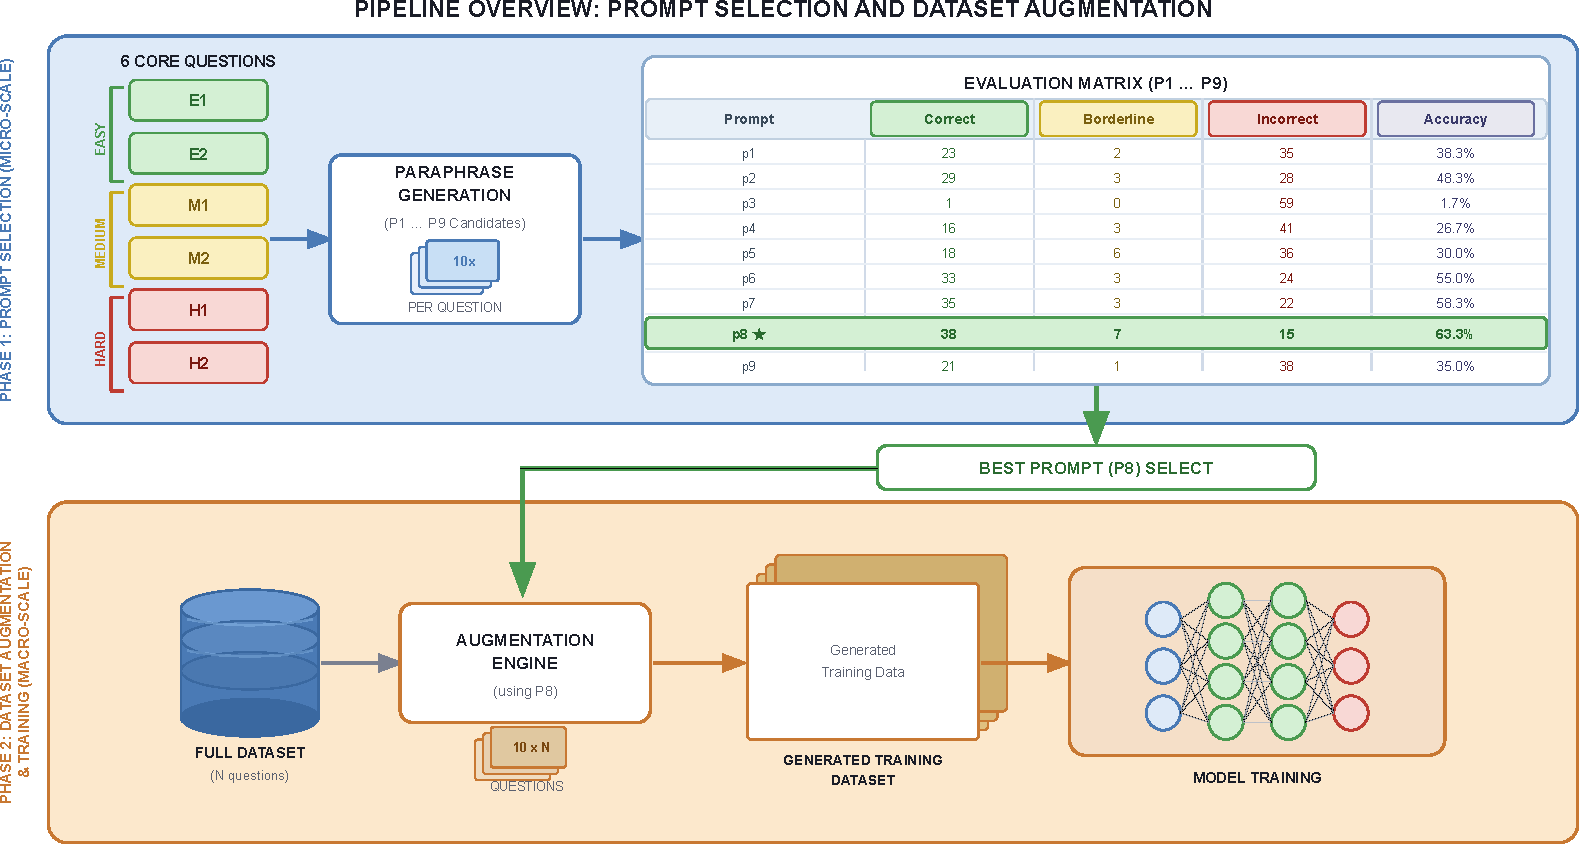
\includegraphics[width=\textwidth]{images/JURSE/pipeline.pdf}
  \caption{Overview of the LLM-based data augmentation pipeline.
  Unique questions from RSVQA-HR are grouped by difficulty and
  passed to LLaMA-2-7B with the selected prompt $p_8$. Ten
  reformulations are generated per question and added to the
  augmented dataset. The example panel illustrates the four
  possible evaluation outcomes for generated questions.}
  \label{fig:pipeline}
\end{figure}
 
It is important to note that no filtering step is
applied to the generated questions beyond the prompt
selection described above. While our manual evaluation
shows that a non-negligible proportion of generated
questions are borderline or incorrect (approximately
30--40\% depending on difficulty level), we chose to
include all generated questions in the augmented
dataset and rely on the model's ability to learn robust
representations despite the noise. This decision is
motivated by the scale of the augmentation: even at a
20\% error rate, the LLM-augmented training set
contains a far greater diversity of valid phrasings
than the original dataset. The impact of this noise
on model performance is analyzed in Section~\ref{sec:chap3_results}.

\begin{table}[ht]
\centering
\small
\caption{Examples of questions generated from the original
question \textit{``Are there more roads than parks?''}
using prompt $p_8$, along with their manual evaluation.}
\label{tab:generated_examples}
\begin{tabular}{ll}
\hline
\textbf{Evaluation} & \textbf{Generated Question} \\
\hline
Correct    & Is the number of roads greater than the number of parks? \\
Correct    & Do roads exceed parks in number? \\
Borderline & Can you name more roads than parks? \\
Incorrect  & Is the total distance of roads longer than the distance of parks? \\
\hline
\end{tabular}
\end{table}


 %============================================================
\section{Experimental Study}
\label{sec:chap3_experiments}
% ============================================================
 
\subsection{Dataset: RSVQA-HR}
\label{sec:chap3_dataset}
 
Our experiments are conducted on the RSVQA-HR
dataset~\cite{lobry2020rsvqa}, the high-resolution
benchmark of the RSVQA family. It uses orthoimagery
at 15\,cm resolution from the USGS data collection,
covering urban areas of the United States. The dataset
consists of 10,659 images and 955,664 question-answer
pairs distributed across four question types: presence
(\textit{e.g.}, \textit{``Is there a road?''}), area
(\textit{e.g.}, \textit{``What is the area covered by
grass?''}), count (\textit{e.g.}, \textit{``How many
buildings are there?''}), and comparison (\textit{e.g.},
\textit{``Are there more roads than parks?''}).
 
The dataset is divided into a training set
(625,340 question-answer pairs), a validation set
(102,843 pairs), test set 1 (222,684 pairs, covering
images similar in distribution to the training set),
and test set 2 (covering a city not seen during
training, used to evaluate geographic generalization).
This structure makes RSVQA-HR particularly well-suited
for evaluating generalization: test set 2 provides
a natural out-of-distribution evaluation that goes
beyond linguistic variation.
 
Following the augmentation procedure described in
Section~\ref{sec:chap3_pipeline}, the LLM-augmented
training set contains 6,878,740 question-answer pairs, 
more than ten times the original size. For
comparison, the back-translation-augmented training
set contains 1,739,794 pairs, as back translation
via three pivot languages (French, German, Chinese)
generates at most three additional versions per
question, with duplicates discarded.
 
\subsection{Experimental Setup}
\label{sec:chap3_setup}
 
\textbf{Model architecture.} Following the findings
of \cite{chappuis2023curse}, we use a dual-encoder
architecture as our RSVQA baseline. The visual branch
consists of a ResNet-152~\cite{he2016resnet} pretrained
on ImageNet and kept frozen during training. The
language branch consists of a
DistilBERT~\cite{sanh2019distilbert} encoder
fine-tuned during training. Visual and textual
representations are fused via point-wise
multiplication, followed by a multilayer perceptron
for answer prediction. This architecture is
representative of the encoder-based RSVQA paradigm
dominant at the time of this work and provides a
clean, reproducible baseline for evaluating the
effect of data augmentation independently of
architectural choices.
 
\textbf{Training conditions.} We train three separate
instances of this model on three different training
sets: the original unaugmented dataset (Original),
the LLM-augmented dataset (LLM-Aug), and the
back-translation-augmented dataset (BT-Aug). All
other hyperparameters are kept identical across
the three conditions to ensure that observed
differences in performance are attributable solely
to the training data.
 
\textbf{Evaluation protocol.} Each model is evaluated
on three test sets: the original test set 1
(Original), the LLM-augmented test set 1 (LLM-Aug),
and the back-translation-augmented test set 1
(BT-Aug). This cross-evaluation design (training
on one distribution, testing on another), allows
us to measure not only in-distribution performance
but also the degree to which each augmentation
strategy produces question distributions that are
genuinely novel and distinct from the original.
Overall accuracy and per-category accuracy are
reported.
 
\subsection{Results and Discussion}
\label{sec:chap3_results}
 
Table~\ref{tab:results} presents the cross-evaluation
results for all three models across all three test sets.
 
\begin{table*}[ht]
\centering
\footnotesize
\caption{Performance comparison of Original, LLM-Aug, and
BT-Aug models across different test sets. Accuracy (\%) per
question type. Avg = average across the three test sets.
Best per training condition in \textbf{bold}.}
\label{tab:results}
\begin{tabularx}{\textwidth}{
  l
  >{\centering\arraybackslash}X
  >{\centering\arraybackslash}X
  >{\centering\arraybackslash}X
  >{\centering\arraybackslash}X
  >{\centering\arraybackslash}X
  >{\centering\arraybackslash}X
  >{\centering\arraybackslash}X
  >{\centering\arraybackslash}X
  >{\centering\arraybackslash}X
  >{\centering\arraybackslash}X
  >{\centering\arraybackslash}X
  >{\centering\arraybackslash}X}
\toprule
& \multicolumn{4}{c}{\textbf{Train: Original}}
& \multicolumn{4}{c}{\textbf{Train: LLM-Aug}}
& \multicolumn{4}{c}{\textbf{Train: BT-Aug}} \\
\cmidrule(lr){2-5}\cmidrule(lr){6-9}\cmidrule(lr){10-13}
\textbf{Type}
& Orig & LLM & BT & Avg
& Orig & LLM & BT & Avg
& Orig & LLM & BT & Avg \\
\midrule
Presence
& 90.39 & 71.31 & 64.02 & 75.24
& \textbf{90.71} & \textbf{90.01} & 63.30 & \textbf{81.34}
& 69.82 & 65.05 & \textbf{68.58} & 67.82 \\
Area
& 81.45 & 23.75 & 64.45 & 56.55
& \textbf{83.88} & \textbf{83.45} & 59.13 & \textbf{75.49}
& 67.45 & 29.03 & \textbf{69.11} & 55.20 \\
Count
& 67.20 & 56.87 & 60.92 & 61.66
& \textbf{67.42} & \textbf{66.71} & \textbf{62.33} & \textbf{65.49}
& 64.57 & 52.02 & 63.57 & 60.39 \\
Comparison
& 89.66 & 56.71 & 70.00 & 72.12
& \textbf{89.91} & \textbf{86.90} & \textbf{67.65} & \textbf{81.49}
& 74.47 & 57.69 & 73.21 & 68.46 \\
\midrule
Overall
& 82.17 & 52.16 & 65.10 & 66.48
& \textbf{82.98} & \textbf{81.77} & 63.10 & \textbf{75.95}
& 69.07 & 50.95 & \textbf{68.37} & 62.80 \\
Average
& 82.78 & 55.70 & 65.13 & 67.87
& \textbf{83.35} & \textbf{81.93} & 63.72 & \textbf{76.33}
& 69.62 & 53.89 & \textbf{68.35} & 63.95 \\
\bottomrule
\end{tabularx}
\end{table*}
 
 
\textbf{In-distribution performance.}
The LLM-Aug model achieves an overall accuracy of
82.98\% on the original test set, slightly above the
Original model (82.17\%). This result is notable: despite
training on a dataset more than ten times larger and
with significantly more diverse phrasings, the LLM-Aug
model does not sacrifice in-distribution accuracy.
This suggests that the generated questions, while
more varied, do not introduce sufficient noise to
degrade performance on the original phrasing
distribution. The BT-Aug model also improves slightly
over the baseline on the original test set (69.07\%
overall), though the gap relative to the LLM-Aug
model is substantial.
 
\textbf{Generalization to augmented phrasings.}
When each model is tested on its own augmented test
set, a clear divergence emerges. The LLM-Aug model
achieves 81.77\% on the LLM-augmented test set,
close to its in-distribution performance, indicating
that the representations it learned are genuinely
robust to paraphrase variation. By contrast, the
Original model drops to 52.16\% on the LLM-augmented
test set, a degradation of nearly 30 percentage
points. This drop confirms two things: first,
that the LLM-generated questions are genuinely
distinct from the originals in terms of surface form;
second, that the Original model has overfit to the
specific phrasings present in the training data and
fails to generalize.
 
\textbf{Question type analysis.}
The area category shows the largest performance gap.
The Original model drops from 81.45\% on the original
test set to 23.75\% on the LLM-augmented test set.
This is consistent with the difficulty grouping
analysis in Section~\ref{sec:chap3_difficulty}: area
questions tend to involve complex spatial descriptions
that are hardest to paraphrase faithfully, meaning
the LLM-generated area questions are the most
linguistically distant from their originals. The
count and comparison categories are more robust,
likely because the core quantitative structure of
these questions is preserved even under paraphrasing.
 
\textbf{Back translation results.}
Both models show a performance drop on the
BT-augmented test set, with the Original model
retaining a slight advantage (approximately 2\%
on overall accuracy). This can be attributed to
two properties of back translation: first, BT-generated
questions tend to remain structurally close to the
originals, so the Original model partially recognizes
them; second, some BT outputs are of lower quality
due to translation errors, which both penalizes the
BT-Aug model during training and introduces harder
test examples. The BT-Aug model performs notably
lower on its own test set than the LLM-Aug model
does on the LLM-augmented test set (68.37\% vs.
81.77\%), suggesting that BT augmentation introduces
more noise and less useful diversity than LLM-based
augmentation.
 
\textbf{Cross-augmentation generalization.}
An interesting pattern emerges when models are
evaluated on a test set produced by a different
augmentation strategy than the one used for training.
All models degrade significantly in this setting,
which confirms that the two augmentation methods
produce genuinely different linguistic distributions.
This result also highlights a limitation of our
evaluation framework: robustness to one type of
paraphrase does not automatically transfer to
robustness to another. Future work could explore
hybrid training strategies that combine multiple
augmentation sources to produce more universally
robust representations.
 
% ============================================================
\section{Conclusion and Limitations}
\label{sec:chap3_conclusion}
% ============================================================
 
In this chapter, we addressed the generalization problem
in RSVQA from a data-centric perspective. We proposed
a question augmentation framework leveraging LLaMA-2-7B
to generate ten semantically equivalent reformulations
of each question in the RSVQA-HR dataset, guided by a
prompt selected through systematic evaluation of nine
candidates across questions of varying linguistic
complexity. Experimental results demonstrate that models
trained on LLM-augmented data achieve higher robustness
to unseen phrasings than models trained on the original
dataset or on back-translation-augmented data, while
maintaining competitive in-distribution accuracy. The
cross-evaluation design further confirms that LLM-generated
questions constitute a genuinely novel and challenging
distribution, distinct from both the original and
back-translated phrasings.
 
\textbf{Limitations.}
Several limitations of this work should be acknowledged.
First, experiments are conducted exclusively on RSVQA-HR,
which covers urban areas of the United States. Whether
the proposed augmentation strategy generalizes to rural
datasets~\cite{lobry2021rsvqaben}, to datasets involving
SAR imagery~\cite{tosato2024sar}, or to geographically
diverse regions remains an open question.
Second, only a single LLM (LLaMA-2-7B) is evaluated.
Larger models in the LLaMA-2 family (13B, 70B) or
other instruction-tuned models may produce higher-quality
paraphrases, particularly for hard questions involving
complex spatial relations. A systematic comparison of
LLM quality and scale on augmentation performance is
left for future work.
Third, the prompt evaluation is conducted on a small
manually reviewed subset. While the selected prompt
($p_8$) achieves the highest accuracy in this evaluation,
the review process does not measure inter-annotator
agreement, and the borderline category introduces
subjectivity into the quality assessment.
Finally, it remains to be verified whether the benefits
of LLM-based augmentation transfer to more recent
generative RSVQA architectures based on large
vision-language models, where the base model already
possesses significant linguistic diversity from
pre-training.
 
\textbf{Perspectives.}
Future work could explore hybrid augmentation strategies
combining LLM-based question generation with image-level
augmentation or answer-aware generation. The compatibility
of the proposed approach with semantic-based RSVQA
methods~\cite{tosato2024segguided} also warrants
investigation. More broadly, this work highlights the
importance of data diversity as a first-class concern
in RSVQA research, complementary to architectural
innovations.
 
While this chapter addressed generalization from
a data perspective, the following chapter investigates
how model architecture itself can be improved to better
exploit the spatial structure present in remote sensing
imagery. Specifically, how segmentation maps can be
used to guide visual attention in RSVQA models.
 